\documentclass[12pt]{article}
\usepackage[utf8]{inputenc}
\usepackage[LGR,T1]{fontenc}
\usepackage[greek,english]{babel}
\usepackage{alphabeta}
\usepackage{listings}
\usepackage{xcolor}
\usepackage{booktabs}
\usepackage{multirow}
\usepackage{graphicx}
\usepackage{amsmath}
\usepackage{float}
\usepackage[unicode]{hyperref}
\usepackage{subcaption}
\usepackage[a4paper, total={17cm, 25cm}]{geometry}
\usepackage{setspace}
\setstretch{1.15}
\usepackage{tikz}
\usepackage{tikz}
\usepackage{caption}
\usepackage{subcaption}
\usepackage{booktabs}

\begin{document}
\setcounter{table}{3}

\section*{Μέρος 2: Εντοπισμός Χωρο-χρονικών Σημείων Ενδιαφέροντος
και Εξαγωγή Χαρακτηριστικών σε Βίντεο Ανθρωπίνων Δράσε
ων}

\subsection*{2.1.1 Ανιχνευτής Harris 3D}

\subsubsection*{Θεωρητική Ερμηνεία}
\hspace{0.6cm}Ο ανιχνευτής Harris 3D αποτελεί γενίκευση του κλασικού ανιχνευτή γωνιών Harris-Stephens στον χωρο-χρόνο. Στόχος της μεθόδου είναι ο εντοπισμός voxels $(x, y, t)$ όπου παρατηρείται έντονη μεταβολή της έντασης $L(x, y, t)$ και στις τρεις διαστάσεις. Τα σημεία ενδιαφέροντος δεν εντοπίζονται απλώς σε χωρικές γωνίες, αλλά σε σημεία όπου η κίνηση αλλάζει κατεύθυνση ή επιταχύνεται (χωροχρονική γωνία). Πιο απλοϊκά, εντοπίζονται χωρικές γωνίες οι οποίες εισέρχονται και εξέρχονται από μια περιοχή παρακολούθησης μέσα σε λίγα frames (χρονική γωνία).

Για την εξαγωγή των σημείων ενδιαφέροντος, αναζητούμε περιοχές όπου και οι τρεις ιδιοτιμές $(\lambda_1, \lambda_2, \lambda_3)$ του δομικού τανυστή είναι μεγάλες. Οι ιδιοτιμές αυτές αντιπροσωπεύουν την ένταση της μεταβολής στις τρεις κατευθύνσεις που ορίζουν τα αντίστοιχα ιδιοδιανύσματα (χώρος-χρόνος).


Η παράμετρος $\sigma$ καθορίζει τη χωρική εξομάλυνση, ενώ η $\tau$ τη χρονική, δηλαδή αναλαμβάνουν την αποθορυβοποίση του βίντεο στις τρεις διαστάσεις. Μεγάλες τιμές του σ εξαλείφουν λεπτομέρειες και υφές σε κάθε frame  ενώ μεγάλες τιμές του $\tau$ τείνουν να εξαλείφουν την απόκριση σε πολύ γρήγορες κινήσεις, εστιάζοντας σε πιο σταθερές δράσεις. Η παράμετρος $s$ καθορίζει την περιοχή ολοκλήρωσης, εξασφαλίζοντας ότι ο τανυστής ενσωματώνει πληροφορία από μια επαρκή γειτονιά γύρω από το voxel.

Αξίζει να σημειωθεί πως σε αντίθεση με τον 2D Harris, στατικά αντικείμενα δεν παράγουν σημεία ενδιαφέροντος, καθώς η χρονική παράγωγος $L_t \approx 0$ οδηγεί σε $\text{det}(M) \approx 0$. Αυτή η διαφορά παρουσιάζεται στην εικόνα 6 που ακολουθεί.

\setcounter{figure}{5}
\begin{figure}[H]
     \centering
     \begin{subfigure}[b]{0.49\textwidth}
         \centering
         \includegraphics[width=\linewidth]{2d_harris.png}
         \caption{Ανιχνευμένα σημεία ενδιαφέροντος (χωρικές γωνίες) από τον ανιχνευτή Harris.}
     \end{subfigure}
     \hfill
     \begin{subfigure}[b]{0.49\textwidth}
         \centering
         \includegraphics[width=\linewidth]{3d_harris.png}
         \caption{Ανιχνευμένα σημεία ενδιαφέροντος (χωροχρονικές γωνίες) από τον ανιχνευτή Harris3D.}
     \end{subfigure}
     \caption{Ανιχνεύεσεις σημείων που πληρούν το κριτήριο γωνιότητας για τον ανιχνευτή Harris και την επέκτασή του στις τρεις διαστάσεις, Harris3D. Ο Harris3D εντοπίζει σημεία που είναι πιο εστιασμένα στις δράσεις, λαμβάνοντας υπόψην και την διάσταση του χρόνου.}
    \label{fig:running_harris_gabor}
\end{figure}


\subsection*{2.1.2 Ανιχνευτής Gabor}

\subsubsection*{Θεωρητική Ερμηνεία}
\hspace{0.6cm}Ο ανιχνευτής Gabor εστιάζει στον εντοπισμό περιοχών των οποίων η ένταση εμφανίζει περιοδικότητα στον χρόνο. Λειτουργεί ως ένα σύστημα επιλεκτικής συχνότητας. Το κριτήριό του ενεργοποιείται όταν η τοπική μεταβολή της έντασης του βίντεο "συντονίζεται" με τη συχνότητα ταλάντωσης $\omega$ του Gabor πυρήνα. Όταν συμβαίνουν τα παραπάνω ο ανιχνευτής αυτός τείνει να παράγει περισσότερα σημεία ενδιαφέροντος (πιο dense) σε σχέση με τον Harris, γεγονός που αυξάνει τον θόρυβο στην τελική αναπαράσταση αν δεν χρησιμοποιηθεί αυστηρό κατώφλι. Αντίθετα, αν η συχνότητα της κίνησης δεν προσεγγίζει την συχνότητα του φίλτου η εύρεση σημείων θα είναι φτωχή.

Η χωρική εξομάλυνση με Gaussian εξασφαλίζει ότι η απόκριση δεν οφείλεται σε μεμονωμένο θόρυβο pixels, αλλά σε συλλογική κίνηση μιας περιοχής με ακτίνα ανάλογη του $\sigma$.

Εστιάζοντας στο κριτήριο σημαντικότητας, αυτό μπορεί να ερμηνευθεί ως η ενέργεια του βίντεο σε μια ζώνη συχνοτήτων γύρω από το ω. Η χρήση του ζεύγους φίλτρων $h_{ev}$ και $h_{od}$  είναι απαραίτητη ώστε όταν ο ένας όρος μηδενιστεί λόγω της φάσης του ο άλλος να είναι διάφορος του μηδενός και ικανός να ανιχνεύσει σημείο ενδιαφέροντος.


\subsection*{2.1.3 Κατωφλιωποίηση και Απόρριψη Περιοχών Χαμηλής Σημαντικότητας}

\hspace{0.6cm}Η επιβολή ενός κατωφλίου $\theta$ στις συναρτήσεις απόκρισης αποσκοπεί στον περιορισμό των σημείων ενδιαφέροντος μόνο σε voxels που φέρουν σημαντική πληροφορία. Με τη διαδικασία αυτή απορρίπτονται οι "ομαλές" περιοχές του βίντεο (background, ενιαίες επιφάνειες), όπου οι παράγωγοι έντασης ή οι αποκρίσεις των φίλτρων οφείλονται κυρίως σε θόρυβο και όχι σε πραγματική χωρο-χρονική δομή. Το θ ρυθμίζεται σε κατάλληλη τιμή ώστε να μην εισάγει μεγάλο αριθμό false positives (αυξάνοντας αχρείαστα το υπολογιστικό κόστος) αλλά και να μην αποτελεί ανυπέρβλητο εμπόδιο το οποίο θα έδινε μια αραιή αναπαράσταση του βίντεο.

Η ανάγκη για διαφορετική αυστηρότητα στο κατώφλι μεταξύ των δύο μεθόδων ερμηνεύεται από την διαφορετική μορφή των κριτηρίων σημαντικότητας:
\begin{itemize}
    \item \textbf{Harris (Ήπιο Κατώφλι):} Η απόκριση $H$ εξαρτάται από την ορίζουσα του τανυστή δομής ($\text{det}(M) \sim \lambda^3$). Σε ομαλές περιοχές όπου οι ιδιοτιμές είναι μικρές, η τιμή του $H$ προσεγγίζει το μηδέν και πολλές φορές γίνεται αρνητική. Συνεπώς, ακόμα και ένα σχετικά μικρό κατώφλι είναι επαρκές για να διαχωρίσει το σήμα από το υπόβαθρο.
    \item \textbf{Gabor (Αυστηρό Κατώφλι):} Η απόκριση $Η$ είναι ένα μέτρο ενέργειας, δηλαδή άθροισμα τετραγώνων, με αποτέλεμσα οι τιμές του να μην λαμβάνουν ποτέ αρνητική τιμή. Επιπλέον λόγω των ταλαντώσεων των πυρήνων Gabor και της Gaussian εξομάλυνσης, τείνει να παρουσιάζει ευρείες αποκρίσεις γύρω από το κύριο γεγονός. Απαιτείται λοιπόν πολύ πιο αυστηρό κατώφλι για να κατασταλούν οι δευτερεύουσες κορυφές.
\end{itemize}

\subsection*{2.1.4 Ανάλυση Τύπου Σημείων, Κλιμάκων και Πολυκλιμακωτής Ανίχνευσης}

\subsubsection*{Σύγκριση Τύπου Σημείων ανά Δράση}
Η πειραματική αξιολόγηση των δύο ανιχνευτών στις κλάσεις \textit{walking, running, handclapping} αναδεικνύει θεμελιώδεις διαφορές στη φύση των ανιχνευόμενων σημείων:

\begin{itemize}
    \item \textbf{Walking/Running:} 
    \begin{itemize}
        \item Ο \textbf{Harris 3D} εντοπίζει σημεία κυρίως στις αρθρώσεις (γόνατα, πέλματα) και στα άκρα του σώματος, εκεί όπου οι χωρικές ακμές του υποκειμένου αλλάζουν απότομα κατεύθυνση στον χρόνο (πάτημα/bounce του ποδιού στο έδαφος). Στο \textit{running}, αναμένεται οι αποκρίσεις να είναι εντονότερες λόγω των υψηλότερων τιμών της χρονικής παραγώγου $L_t$.
        \item Ο \textbf{Gabor} εστιάζει στην περιοδικότητα του διασκελισμού. Τα σημεία είναι πιο ομοιόμορφα κατανεμημένα κατά μήκος της τροχιάς των μελών του σώματος, καθώς ο ανιχνευτής "συντονίζεται" με τη συχνότητα της ταλάντωσης τους.
    \end{itemize}

\begin{figure}[H]
     \centering
     \begin{subfigure}[b]{0.49\textwidth}
         \centering
         \includegraphics[width=\linewidth]{part2_imgs/hs_running_frame16.png}
         \caption{Harris Detector (frame16)}
     \end{subfigure}
     \hfill
     \begin{subfigure}[b]{0.49\textwidth}
         \centering
         \includegraphics[width=\linewidth]{part2_imgs/gs_running_frame16.png}
         \caption{Gabor Detector (frame16)}
     \end{subfigure}
     \caption{Σύγκριση ανίχνευσης σημείων ενδιαφέροντος στο βίντεο person01\_running\_d1\_uncomp.}
    \label{fig:running_harris_gabor}
\end{figure}


\begin{figure}[H]
     \centering
     \begin{subfigure}[b]{0.49\textwidth}
         \centering
         \includegraphics[width=\linewidth]{part2_imgs/hs_walking_frame37.png}
         \caption{Harris Detector (frame37)}
     \end{subfigure}
     \hfill
     \begin{subfigure}[b]{0.49\textwidth}
         \centering
         \includegraphics[width=\linewidth]{part2_imgs/gb_walking_frame37.png}
         \caption{Gabor Detector (frame37)}
     \end{subfigure}
     \caption{Σύγκριση ανίχνευσης σημείων ενδιαφέροντος στα βίντεο και person04\_walking\_d1\_uncomp.}
    \label{fig:walking_harris_gabor}
\end{figure}


    \item \textbf{Handclapping:} 
    \begin{itemize}
        \item Ο \textbf{Harris} ανιχνεύει τα σημεία επαφής των παλαμών, καθώς κατά την κρούση των χεριών (figure 9 (a)) παρατηρείται η μέγιστη μεταβολή της έντασης σε όλες τις διαστάσεις (χωρική σύγκλιση και χρονική κρούση). Με άλλα λόγια εμφανίζεται έντονη χρωματική αντίθεση μεταξύ χεριών και μαύρης μπλούζας και απότομη αλλαγή κατεύθυνσης.
        \item Το χειροκρότημα χαρακτηρίζεται από ισχυρή περιοδικότητα. Επομένως, το κριτήριο σημαντικότητας του \textbf{Gabor} διατηρεί ψηλές τιμές απόκρισης καθόλη την διάρκεια της τροχιάς των χεριών (figure 9 (a)(β)), άρα και αυξημένο εντοπισμό σημείων. Απαραίτητη προυπόθεση η συχνότητα κίνησης να προσεγγίζει την συχνότητα του φίλτρου.
    \end{itemize}
\begin{figure}[H]
     \centering
     \begin{subfigure}[b]{0.49\textwidth}
         \centering
         \includegraphics[width=\linewidth]{part2_imgs/hs_hnd_frame26.png}
         \caption{Harris Detector (frame26)}
     \end{subfigure}
     \hfill
     \begin{subfigure}[b]{0.49\textwidth}
         \centering
         \includegraphics[width=\linewidth]{part2_imgs/gb_hnd_frame12.png}
         \caption{Gabor Detector (frame12)}
     \end{subfigure}
     \caption{Σύγκριση ανίχνευσης σημείων ενδιαφέροντος στο βίντεο person01\_handclapping\_d2\_uncomp.}
    \label{fig:handclapping_harris_gabor}
\end{figure}

\end{itemize}


\subsection*{Οπτικοποίηση Συναρτήσεων Σημαντικότητας H}

\begin{itemize}

    \item \textbf{Ανιχνευτής Harris 3D (figure 10 - Αριστερή στήλη:} Η συνάρτηση εμφανίζει υψηλή επιλεκτικότητα. Το υπόβαθρο είναι σχεδόν μηδενικό, ενώ η απόκριση εντοπίζεται με μεγάλη ακρίβεια στο σημείο της χωρο-χρονικής ασυνέχειας, για παράδειγμα τη στιγμή και το σημείο της κρούσης των χεριών. Στο σημείο αυτό είναι προφανής η ύπαρξη έντονων παραγώγων και στις τρεις διαστάσεις.
 
    \item \textbf{Ανιχνευτής Gabor (figure 10 - Δεξιά στήλη:} Η συνάρτηση απόκρισης παρουσιάζει μια πιο διάχυτη κατανομή γύρω από τις περιοχές δράσης. Στην δράση handclapping, παρατηρούμε ότι ο ανιχνευτής ενεργοποιείται γύρω από τα δύο χέρια, καθώς η χρονική συχνότητα της κίνησής τους συντονίζεται με τον πυρήνα Gabor. Η παρουσία θολούρας στο υπόβαθρο οφείλεται στην ενέργεια που συλλέγουν τα φίλτρα (στο άθροισμα των τεταργώνων) από ασθενέστερες χωρο-χρονικές μεταβολές, γεγονός που υποδεικνύει την χρήση αυστηρότερου κατωφλίου.
    
\end{itemize}

\begin{figure}[H]
    \centering
    % --- 1η Σειρά ---
    \begin{subfigure}[b]{0.49\textwidth}
        \centering
        \includegraphics[width=\linewidth]{part2_imgs/hs_H_frame26.png}
        %\caption{Λεζάντα 1}
    \end{subfigure}
    \hfill
    \begin{subfigure}[b]{0.49\textwidth}
        \centering
        \includegraphics[width=\linewidth]{part2_imgs/gb_H_frame12.png}
        %\caption{Λεζάντα 2}
    \end{subfigure}

    \vspace{0.5cm} % Προσθέτει λίγο κάθετο κενό μεταξύ των σειρών

    % --- 2η Σειρά ---
    \begin{subfigure}[b]{0.48\textwidth}
        \centering
        \includegraphics[width=\linewidth]{part2_imgs/hs_running_H_frame16.png}
        %\caption{Λεζάντα 3}
    \end{subfigure}
    \hfill
    \begin{subfigure}[b]{0.48\textwidth}
        \centering
        \includegraphics[width=\linewidth]{part2_imgs/gb_running_H_frame16.png}
        %\caption{Λεζάντα 4}
    \end{subfigure}

    \vspace{0.5cm}

    % --- 3η Σειρά ---
    \begin{subfigure}[b]{0.48\textwidth}
        \centering
        \includegraphics[width=\linewidth]{part2_imgs/hs_walking_H_frame37.png}
        %\caption{Λεζάντα 5}
    \end{subfigure}
    \hfill
    \begin{subfigure}[b]{0.48\textwidth}
        \centering
        \includegraphics[width=\linewidth]{part2_imgs/gb_walking_H_frame37.png}
        %\caption{Λεζάντα 6}
    \end{subfigure}

    \caption{Οπτικοποίηση της Η για τους δύο ανιχνευτές στα frames των figures 7 και 8.}
    \label{fig:six_images}
\end{figure}
Συνοπτικά ο Gabor λειτουργεί ως ανιχνευτής "περιοχών κίνησης", ενώ ο Harris ως ανιχνευτής "σημειακών συμβάντων".

\subsubsection*{Επίδραση Χωρικών και Χρονικών Κλιμάκων και Περιβάλλοντος}
Η αλληλεπίδραση με το Dataset KTH φανέρωσε την ύπαρξη βίντεο σε διαφορετικά περιβάλλοντα και με διαφορετικές συνθήκες λήψης. Πιο συγκεκριμένα οι δραστηριότητες έχουν καταγραφεί σε διαφορετικούς χώρους (εσωτερικούς και υπαίθριους), με διαφορετικά ρούχα και από διαφορετικές αποστάσεις/κλίμακες. Η διαφοροποίηση στις συνθήκες απαιτεί και την κατάλληλη ρύθμιση των παραμέτρων στους ανιχνευτές.

Πιο συγκερκιμένα οι παράμετροι $(\sigma, \tau)$ καθορίζουν το "παράθυρο" παρατήρησης της δράσης. Η επιλογή τους επηρεάζεται άμεσα από τις συνθήκες λήψης:

\begin{enumerate}
    \item \textbf{Απόσταση και Zoom (Χωρική Κλίμακα $\sigma$):} Όταν η κάμερα βρίσκεται μακριά ή σε κατάσταση zoom-out, το υποκείμενο καταλαμβάνει λιγότερα pixels, άρα οι λεπτομέρειες (π.χ. παλάμες) απαιτούν μικρότερο $\sigma$. Αντίθετα, σε κοντινά πλάνα (zoom-in), απαιτείται μεγαλύτερο $\sigma$ για την κάλυψη των δομών, ώστε ο τανυστής δομής $M$ να μην επηρεάζεται από τοπικό θόρυβο υφής.
    \item \textbf{Ταχύτητα Δράσης (Χρονική Κλίμακα $\tau$):} Δράσεις όπως το \textit{running} απαιτούν μικρότερο $\tau$ για την αποφυγή υπερβολικής χρονικής εξομάλυνσης που θα "θόλωνε" την κίνηση. Στο \textit{walking}, ένα μεγαλύτερο $\tau$ βοηθά στον διαχωρισμό της σκόπιμης κίνησης από τον τυχαίο θόρυβο.
    \item \textbf{Περιβάλλον και Εμφάνιση:} 
    \begin{itemize}
        \item \textbf{Εσωτερικός/Εξωτερικός χώρος:} Στον εξωτερικό χώρο, οι μεταβολές του φωτισμού μπορούν να προκαλέσουν ψευδείς παραγώγους $L_t$.
        \item \textbf{Ενδυμασία:} Ρούχα με χαμηλή αντίθεση ως προς το υπόβαθρο (π.χ. σκούρα ρούχα σε σκιερό μέρος) μειώνουν το μέτρο των παραγώγων $L_x, L_y$. Ο Harris είναι πιο ευάλωτος σε αυτό, ενώ ο Gabor, βασιζόμενος στη συχνότητα, μπορεί να ανιχνεύσει την κίνηση ακόμα και με ασθενέστερο contrast.
    \end{itemize}
\end{enumerate}

Συνεπώς προκειμένου ο ανιχνευτής να είναι προσαρμοστικός σε όλες αυτές τις αλλαγές (οι οποίες ενδέχεται να συμβαίνουν κατά την διάρκεια ενός βίντεο) επιλέχθηκε η υλοποίηση των αλγορίθμων και στην πολυκλιμακωτή εκδοχή τους.

\subsubsection*{Πολυκλιμακωτή Ανίχνευσης}
Η πολυκλιμακωτή μέθοδος αναμένεται να ανιχνεύει ταυτόχρονα σημεία ενδιαφέροντος διαφορετικών διαστάσεων λόγω της μεταβαλλόμενης τιμής του σ. Η τελική επιλογή των σημείων καθορίζεται από το αν  η κανονικοποιημένη Λαπλασιανή εμφανίζει τοπικό μέγιστο στο σημείο αυτό. Επιπλέον περιμένουμε να επιτρέπει την ταυτόχρονη ανίχνευση δράσεων που συμβαίνουν σε διαφορετικές αποστάσεις από την κάμερα ή με διαφορετικές ταχύτητες στο ίδιο πλάνο, καθιστώντας το σύστημα πιο εύρωστο σε ρεαλιστικά σενάρια βίντεο.

\begin{figure}[H]
     \centering
     \begin{subfigure}[b]{0.49\textwidth}
         \centering
         \includegraphics[width=\linewidth]{part2_imgs/mshs_frame45.png}
         \caption{Multiscale Harris Detector (frame45)}
     \end{subfigure}
     \hfill
     \begin{subfigure}[b]{0.49\textwidth}
         \centering
         \includegraphics[width=\linewidth]{part2_imgs/msgb_frame45.png}
         \caption{Multiscale Gabor Detector (frame45)}
     \end{subfigure}
     \caption{Σύγκριση πολυκλιμακωτών ανιχνευτών στο βίντεο person01\_handclapping\_d2\_uncomp.}
    \label{fig:multiscale_comparison}
\end{figure}

Έπειτα από πειραματικές δοκιμές και απεικονίσεις (figure 11}) φαίνεται πως η πολυκλιμακωτή υλοποίηση του Harris εμφανίζει τα περισσότερα από τα προτερήματα που αναφέραμε παραπάνω. Πιο συγκεκριμένα παρατηρούμε ότι καταφέρνει να εντοπίσει ταυτόχρονα σημεία κίνησης που ανήκουν σε διαφορετικές χωρικές κλίμακες: μικρότερα σημεία στα \textbf{χέρια} (ταχεία κίνηση, λεπτομερής δομή) και μεγαλύτερα σημεία στο \textbf{κεφάλι} ή τον κορμό (πιο συμπαγής δομή). Η ικανότητά του να κλειδώνει στην ιδανική κλίμακα μέσω της κανονικοποιημένης Λαπλασιανής τον καθιστά εξαιρετικά εύρωστο. 

Αντίθετα η απόδοση του ανιχνευτή Gabor παρουσιάζει κατακόρυφη πτώση. Παρατηρούμε πλήρη αποτυχία εντοπισμού ενδιαφέροντος πάνω στο υποκείμενο, ενώ εμφανίζονται πολυάριθμα ψευδή σημεία στο υπόβαθρο. Το αποτέλεσμα αυτό δεν αποτελεί έκπληξη, καθώς ο πειραματισμός στα προηγούμενα βήματα με μεμονωμένες κλίμακες $(\sigma, \tau)$ είχε ήδη υποδείξει ότι ο Gabor απαιτεί εξαιρετικά σχολαστική ρύθμιση. Σε μια πολυκλιμακωτή υλοποίηση, πολλές από τις επιλεγμένες κλίμακες $(\sigma_i, \tau_j)$ ενδέχεται να βρίσκονται τελείως εκτός του φάσματος της πραγματικής κίνησης. Αξίζει να σημειωθεί τέλος ότι η λογική του LoG σαν κριτήριο επιλογής της κλίμακας είναι βελτιστοποιημένη για δομές τύπου blob ή corner ενώ ο Gabor παράγει αποκρίσεις ενέργειας που συχνά δεν έχουν σαφή κορυφή στον χώρο των κλιμάκων.

\subsubsection*{Παρατηρήσεις επί της Υλοποίησης σε Python}

\hspace{0.6cm}Λόγω διαγώνιου πίνακα $\Sigma$, η 3D συνέλιξη με Gaussian φίλτρο υλοποιείται ως σειρά τριών διαδοχικών 1D συνελίξεων (\texttt{convolve1d}) στους άξονες $x, y, t$. Αυτή η προσέγγιση μειώνει δραστικά το υπολογιστικό κόστος (από Ο($Ν^3$) σε Ο(3Ν)) και τις απαιτήσεις σε μνήμη RAM.

Για τον αποδοτικό εντοπισμό των σημείων ενδιαφέροντος χρησιμοποιήθηκε η \texttt{maximum\_filter}, η οποία επιτρέπει τον ταχύ προσδιορισμό των τοπικών κορυφών, σε γειρονίες 3x3x3 στην 3D δομή της συνάρτησης απόκρισης $H$. Δεν προτιμήθηκε η πρόταση της εκφώνησης και εύρεση των 500-600 μεγαλύτερων τιμών της Η καθώς αυτό οδηγούσε στην κατανάλωση όλων των "διαθέσιμων" σημείων στις χωρο-χρονικές περιοχές των ολικών μεγίστων αφήνοντας ελάχιστα σημεία για την υπόλοιπη "έκταση" του βίντεο. Αυτό έχει προφανώς σαν αποτέλσμα η δράση να μην περιγράφεται εν τέλει καθολικά.

Τέλος ενσωματώθηκε κώδικας αυτοματοποιημένης δημιουργίας αρχείων GIF (μέσω της \texttt{imageio}), ο οποίος μετατρέπει τις ακολουθίες πλαισίων ανίχνευσης σε κινούμενη εικόνα. Αυτό επιτρέπει τη διαισθητική και συνολική εποπτεία της χρονικής συνέπειας των ανιχνευτών σε ολόκληρη τη διάρκεια του σήματος.


\section*{2.2 Χωρο-χρονικοί Ιστογραφικοί Περιγραφητές}

\subsection*{Περιγραφητής HOG}
\hspace{0.6cm}Ο περιγραφητής HOG εστιάζει στην αναπαράσταση της τοπικής μορφής και εμφάνισης ενός αντικειμένου, υπολογίζοντας την κατανομή των διευθύνσεων της κλίσης στην εικόνα. Είναι ιδιαίτερα ισχυρός στην περιγραφή περιγραμμάτων και υφής, ενώ παρουσιάζει αξιοσημείωτη ανοχή σε μεταβολές φωτεινότητας, καθώς βασίζεται σε σχετικές διαφορές εντάσεων. Ωστόσο, το κύριο μειονέκτημά του είναι ότι πρόκειται για έναν στατικό περιγραφητή και δεν φέρει πληροφορία για τη δυναμική της κίνησης, με αποτέλεσμα να μην μπορεί να διακρίνει μεταξύ δύο διαφορετικών δράσεων αν αυτές έχουν παρόμοια στιγμιαία γεωμετρική δομή.

\subsection*{Περιγραφητής HOF}
\hspace{0.6cm}Ο περιγραφητής HOF συμπληρώνει την πληροφορία της εμφάνισης συλλαμβάνοντας την τοπική κίνηση μέσω της οπτικής ροής. Αντί για τις χωρικές παραγώγους, ομαδοποιεί τις κατευθύνσεις των διανυσμάτων μετατόπισης μεταξύ διαδοχικών πλαισίων. Είναι απαραίτητος για την αναγνώριση δράσεων, καθώς μπορεί να περιγράψει το πώς κινείται ένα αντικείμενο ανεξάρτητα από την εμφάνισή του (π.χ. χρώμα ρούχων). Στις αδυναμίες του συγκαταλέγεται η ευαισθησία στον θόρυβο των αλγορίθμων οπτικής ροής και η αδυναμία περιγραφής στατικών στοιχείων του περιβάλλοντος που μπορεί να είναι κρίσιμα για το context της δράσης.

\subsection*{Συνδυαστικός Περιγραφητής HOG-HOF}
\hspace{0.6cm}Η συνένωση των HOG και HOF δημιουργεί μια ενιαία χωρο-χρονική υπογραφή που αξιοποιεί τα συμπληρωματικά τους πλεονεκτήματα. 
Η στατική πληροφορία εμφάνισης και υφής του HOG εμπλουτίζεται με τη δυναμική της κίνησης που συλλαμβάνει ο HOF μέσω της οπτικής ροής. 
Ο συνδυαστικός αυτός περιγραφητής επιτυγχάνει ανώτερη διακριτική ικανότητα, καθώς μπορεί να ταυτοποιήσει δράσεις με παρόμοια 
στιγμιαία γεωμετρία αλλά διαφορετική χρονική εξέλιξη, εξασφαλίζοντας αυξημένη ακρίβεια στην αναγνώριση προτύπων.

\subsection*{Παρατηρήσεις επί της Υλοποίησης σε Python}
\hspace{0.6cm}Για τον υπολογισμό της οπτικής ροής χρησιμοποιήθηκε ο αλγόριθμος \texttt{DualTVL1OpticalFlow}, ο οποίος προσφέρει υψηλή ακρίβεια στον εντοπισμό της κίνησης, απαιτώντας όμως μετατροπή των εικόνων σε τύπο \texttt{uint8} (εύρος 0-255) σύμφωνα με τις προδιαγραφές της OpenCV.

Για κάθε σημείο ενδιαφέροντος ορίστηκε μια περιοχή μεγέθους $4\sigma \times 4\sigma$, λαμβάνοντας πρόνοια για τα όρια της εικόνας (\texttt{y\_min}, \texttt{y\_max} κ.λπ.) ώστε να αποφευχθούν σφάλματα προσπέλασης.

Ο περιγραφητής HOG-HOF προκύπτει από τη συνένωση των δύο επιμέρους διανυσμάτων, προσφέροντας μια ολοκληρωμένη χωρο-χρονική υπογραφή για κάθε σημείο.


\subsection*{Bonus: Οπτικοποίηση Πεδίων και Συμπεράσματα}
Παρόλο που δεν ζητήθηκε ρητά, προχωρήσαμε στην οπτικοποίηση του πεδίου παραγώγων και του πεδίου ροής για το βίντεο \texttt{person01\_handclapping}, εξάγοντας αντίστοιχα αρχεία GIF για συνολική εποπτεία.
\begin{itemize}
    \item \textbf{Derivative Field:} Τα βέλη επικεντρώνονται στο περίγραμμα του υποκειμένου, επιβεβαιώνοντας ότι ο HOG θα κωδικοποιήσει τη σιλουέτα του ανθρώπου.
    \item \textbf{Flow Field:} Παρατηρείται έντονη συγκέντρωση διανυσμάτων στην περιοχή των χεριών κατά τη διάρκεια της δράσης, αποδεικνύοντας ότι ο HOF αποτυπώνει επιτυχώς τη συχνότητα και τη φορά του χειροκροτήματος. Τα βέλη στο backgound δεν αποτελούν σε καμία περίπτωση έκπληξη, αφού στο συγκεκριμένο βίντεο εκτελείται περιοδικό zoom-in, zoom-out της κάμερας οδηγώντας σε φαινόμενη κίνηση του υποβάθρου προς το κέντρο (zoom-out) και προς τα άκρα (zoom-in).
\end{itemize}
Η οπτικοποίηση αυτή λειτούργησε ως εργαλείο επαλήθευσης της ορθότητας των περιγραφητών, διασφαλίζοντας ότι η πληροφορία που τροφοδοτείται στα ιστογράμματα είναι αντιπροσωπευτική της φυσικής δράσης.

\begin{figure}[H]
     \centering
     \begin{subfigure}[b]{0.49\textwidth}
         \centering
         \includegraphics[width=\linewidth]{part2_imgs/vsl_der_frame49.png}
         \caption{Derivative field (frame49)}
     \end{subfigure}
     \hfill
     \begin{subfigure}[b]{0.49\textwidth}
         \centering
         \includegraphics[width=\linewidth]{part2_imgs/vsl_flow_frame49.png}
         \caption{Flow field (frame49)}
     \end{subfigure}
     \caption{Σύγκριση πεδίων ανιχνευτών HOG (derivative field) και HOF (flow field)}
    \label{fig:hog_hof_visualization}
\end{figure}


\section*{2.3 Κατάταξη Δράσεων με Bag of Visual Words και SVM}

\subsection*{Τεχνικές Παρατηρήσεις Υλοποίησης}
\subsubsection*{Συνάρτηση FeatureExtraction και Δομή Δεδομένων}
\hspace{0.6cm}Η συνάρτηση \texttt{FeatureExtraction} υλοποιεί τον διαχωρισμό σε σύνολα εκπαίδευσης και δοκιμής μέσω του flag \texttt{is\_train}, το οποίο ελέγχει αν το εκάστοτε βίντεο περιλαμβάνεται στις προκαθορισμένες λίστες. Η έξοδος results είναι ένα λεξικό του οποίου η προσπέλαση έχει την μορφή \texttt{results[det\_name][desc\_name]}. Για κάθε συνδυασμό αποθηκεύονται λίστες (\texttt{train\_desc}, \texttt{test\_desc}) που περιέχουν 2D πίνακες με τους περιγραφητές κάθε βίντεο (#videos x feature dimension), καθώς και οι αντίστοιχες ετικέτες (\texttt{labels}). Σχεδιαστικά, επιλέχθηκε η προσπέλαση ανά βίντεο ως εξωτερικό loop, ώστε κάθε αρχείο να φορτώνεται στη μνήμη μόνο μία φορά για τον υπολογισμό όλων των ανιχνευτών και περιγραφητών, βελτιώνοντας σημαντικά την ταχύτητα επεξεργασίας και μειώνοντας το I/O. Τέλος, λόγω της υπολογιστικής πολυπλοκότητας της διαδικασίας, τα εξαχθέντα χαρακτηριστικά αποθηκεύονται μόνιμα στον δίσκο μέσω της βιβλιοθήκης \texttt{pickle}.

\subsubsection*{Πειραματική Διαδικασία και Αξιολόγηση}
\hspace{0.6cm}Το κύριο μέρος του κώδικα υλοποιεί τα πειράματα για την αξιολόγηση των εννέα συνολικά συνδυασμών. Για κάθε ζεύγος, οι περιγραφητές τροφοδοτούνται στη συνάρτηση \texttt{bag\_of\_words} για τη δημιουργία της BoVW αναπαράστασης και στη συνέχεια εκπαιδεύεται ο SVM ταξινομητής μέσω της \texttt{svm\_train\_test}. Η διαδικασία καταλήγει στην παραγωγή μιας συγκεντρωτικής αναφοράς που περιλαμβάνει το ποσοστό ακρίβειας (\textit{accuracy}) και τον πίνακα σύγχυσης (\textit{confusion matrix}) για κάθε περίπτωση, παρέχοντας τα απαραίτητα δεδομένα για τη σύγκριση της αποδοτικότητας των μεθόδων.

\subsection*{Ανάλυση και Ερμηνεία Αποτελεσμάτων}
Στον Table 4 και στα figures 13, 14 και 15 παρουσιάζονται οι επιδόσεις των εννέα συνδυασμών ανιχνευτή-περιγραφητή για τις δράσεις του KTH.

\subsubsection*{Σύγκριση Ανιχνευτών (Harris vs. Gabor)}
\hspace{0.6cm}Οι ανιχνευτές \texttt{Harris} και \texttt{MultiScale-Harris} παρουσιάζουν σαφή υπεροχή, αγγίζοντας ακρίβεια έως και 92\%. Αυτό οφείλεται στο γεγονός ότι οι ανιχνευτές αυτοί εντοπίζουν σταθερά σημεία με έντονη μεταβολή έντασης σε όλες τις κατευθύνσεις (γωνίες/δομές), τα οποία στο KTH αντιστοιχούν στα άκρα του σώματος που εκτελούν την κίνηση. Αντίθετα, ο \texttt{Gabor-Detector} υστερεί σημαντικά (67\% με HOG), καθώς η απόδοσή του εξαρτάται άμεσα από τη λεπτομερή ρύθμιση των παραμέτρων $\sigma$ και $\tau$ ώστε να συντονιστεί με τη συχνότητα της κίνησης. Επειδή οι δράσεις του dataset εκτελούνται με διαφορετική συχνότητα οι fixed παράμετροι δεν είναι ιδανικές για ολες τις περιπτώσεις με αποτέλεσμα ο Gabor να ανιχνεύει θόρυβο ή να αγνοεί κρίσιμα χωροχρονικά σημεία ενδιαφέροντος, οδηγώντας σε μεγάλες αστοχίες, όπως η σύγχυση μεταξύ \textit{walking} και \textit{handclapping}.

\subsubsection*{Αξιολόγηση Περιγραφητών (HOG, HOF, HOG-HOF)}
 \hspace{0.6cm}Ο HOG επιτυγχάνει εξαιρετικά αποτελέσματα, υποδεικνύοντας ότι η στατική εμφάνιση και η στάση του σώματος στις συγκεκριμένες (αυστηρά ορισμένες καιι απλές) δράσεις είναι ιδιαίτερα διακριτή. Για παράδειγμα, η έκταση των χεριών στο χειροκρότημα διαφέρει γεωμετρικά από τη στάση κατά το περπάτημα.

Παρατηρείται ότι ο συνδυαστικός περιγραφητής HOG-HOF αποδίδει συχνά χειρότερα από τον απλό HOG. Μια προσπάθεια ερμηνείας αυτού του φαινομένου είναι πως η συνένωση των διανυσμάτων αυξάνει σημαντικά τη διάσταση του χαρακτηριστικού, με αποτέλεσμα ο SVM ταξινομητής να δυσκολεύεται να βρει το βέλτιστο υπερεπίπεδο διαχωρισμού δεδομένου του πολύ μικρού δείγματος εκπαίδευσης. Επιπλέον, λόγω της φύσης του KTH, η πληροφορία κίνησης που αποτυπώνει ο HOF μπορεί να είναι πλεονασματική όταν η εμφάνιση που αποτυπώνει ήδη ο HOG είναι ήδη επαρκής, εισάγοντας τελικά θόρυβο στη διαδικασία.

\subsubsection*{Ενδεικνύμενοι συνδυασμοί Ανιχνευτή-Περιγραφητή}
\hspace{0.6cm}Συνολικά, ο συνδυασμός Harris-HOG αναδεικνύεται ως ο πλέον ενδεδειγμένος για δράσεις με διακριτή γεωμετρία, καθώς η ικανότητα του Harris να εντοπίζει χωρικές γωνίες συμπληρώνεται ιδανικά από την περιγραφή της τοπικής μορφής που προσφέρει ο HOG. 

Από την άλλη πλευρά, ο Gabor-Detector παρουσιάζει συνάφεια με τον HOF, καθώς και οι δύο μηχανισμοί επικεντρώνονται στο χρονικό σκέλος του σήματος: ο Gabor λειτουργεί ως χωροχρονικό φίλτρο συχνότητας που κλειδώνει σε περιοδικές κινήσεις, ενώ ο HOF κωδικοποιεί την κατεύθυνση αυτής της κίνησης. Παρά την πτώση της απόδοσης του Gabor λόγω παραμετροποίησης, η χρήση του HOF αντί του HOG βελτιώνει τα αποτελέσματά του (από 0.67 σε 0.83), επιβεβαιώνοντας ότι όταν ένας ανιχνευτής βασίζεται στη χρονική μεταβολή, η περιγραφή της οπτικής ροής είναι πιο αντιπροσωπευτική από τη στατική εμφάνιση

\subsubsection*{Σφάλματα Ταξινόμησης}
Βάσει των confusion matrices, η κύρια αστοχία εντοπίζεται μεταξύ των κλάσεων \textit{running} και \textit{walking} για τον Harris ενώ για τον Gabor η αναγνώριση της δράσης walking είναι το αδύναμο σημείο. 

Η πρώτη παρατήρηση είναι αναμενόμενη, καθώς οι δύο δράσεις προσφέρουν ίδια σημεία ενδιαφέροντος προς τον Harris (πέλμα κατά το πάτημα στο έδαφος) και μοιράζονται παρόμοια γεωμετρικά χαρακτηριστικά (HOG) και κατευθύνσεις οπτικής ροής (HOF), με τη βασική τους διαφορά να έγκειται στην ταχύτητα εκτέλεσης, πληροφορία που συχνά χάνεται με την χρήση ιστογραμμάτων και BoW.

Η δεύτερη παρατήρηση μπορεί να οφείλεται στο γεγονός οτι στην δική μας περίπτωση οι παράμετροι έχουν ρυθμιστεί ώστε να προσεγγίζουν τις συχνότητες των δράσεων running και clapping (που ενδεχομένως μοιάζουν μεταξύ τους) αλλά όχι και αυτή της δράσης walking που μπορεί να θεωρηθεί μικρότερη.

\begin{table}[H]
\centering
\begin{tabular}{@{}llc@{}}
\toprule
\textbf{Ανιχνευτής (Detector)} & \textbf{Περιγραφητής (Descriptor)} & \textbf{Ακρίβεια (Accuracy)} \\ \midrule
\multirow{3}{*}{Harris}          & HOG                                & \textbf{0.92}                \\
                                 & HOF                                & \textbf{0.92}                \\
                                 & HOG-HOF                            & 0.83                         \\ \midrule
\multirow{3}{*}{MultiScale-Harris} & HOG                              & \textbf{0.92}                \\
                                 & HOF                                & 0.83                         \\
                                 & HOG-HOF                            & 0.83                         \\ \midrule
\multirow{3}{*}{Gabor-Detector}  & HOG                                & 0.67                         \\
                                 & HOF                                & 0.83                         \\
                                 & HOG-HOF                            & 0.75                         \\ \bottomrule
\end{tabular}
\caption{Αποτελέσματα Accuracy για τους συνδυασμούς Ανιχνευτών και Περιγραφητών στο KTH dataset.}
\label{tab:results_kth}
\end{table}


\begin{figure}[H]
     \centering
     % --- Confusion Matrix 1: Harris + HOG ---
     \begin{subfigure}[b]{0.3\textwidth}
         \centering
         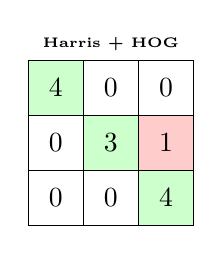
\begin{tikzpicture}[scale=0.7]
            \draw[fill=green!20] (0,2) rectangle (1,3) node[pos=.5] {4};
            \draw[fill=white] (1,2) rectangle (2,3) node[pos=.5] {0};
            \draw[fill=white] (2,2) rectangle (3,3) node[pos=.5] {0};
            
            \draw[fill=white] (0,1) rectangle (1,2) node[pos=.5] {0};
            \draw[fill=green!20] (1,1) rectangle (2,2) node[pos=.5] {3};
            \draw[fill=red!20] (2,1) rectangle (3,2) node[pos=.5] {1};
            
            \draw[fill=white] (0,0) rectangle (1,1) node[pos=.5] {0};
            \draw[fill=white] (1,0) rectangle (2,1) node[pos=.5] {0};
            \draw[fill=green!20] (2,0) rectangle (3,1) node[pos=.5] {4};
            
            \node at (1.5,3.3) {\tiny \textbf{Harris + HOG}};
         \end{tikzpicture}
         \caption{Accuracy: 0.92}
     \end{subfigure}
     \hfill
     % --- Confusion Matrix 2: Harris + HOF ---
     \begin{subfigure}[b]{0.3\textwidth}
         \centering
         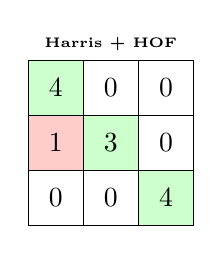
\begin{tikzpicture}[scale=0.7]
            \draw[fill=green!20] (0,2) rectangle (1,3) node[pos=.5] {4};
            \draw[fill=white] (1,2) rectangle (2,3) node[pos=.5] {0};
            \draw[fill=white] (2,2) rectangle (3,3) node[pos=.5] {0};
            
            \draw[fill=red!20] (0,1) rectangle (1,2) node[pos=.5] {1};
            \draw[fill=green!20] (1,1) rectangle (2,2) node[pos=.5] {3};
            \draw[fill=white] (2,1) rectangle (3,2) node[pos=.5] {0};
            
            \draw[fill=white] (0,0) rectangle (1,1) node[pos=.5] {0};
            \draw[fill=white] (1,0) rectangle (2,1) node[pos=.5] {0};
            \draw[fill=green!20] (2,0) rectangle (3,1) node[pos=.5] {4};
            
            \node at (1.5,3.3) {\tiny \textbf{Harris + HOF}};
         \end{tikzpicture}
         \caption{Accuracy: 0.92}
     \end{subfigure}
     \hfill
     % --- Confusion Matrix 3: Harris + HOG-HOF ---
     \begin{subfigure}[b]{0.3\textwidth}
         \centering
         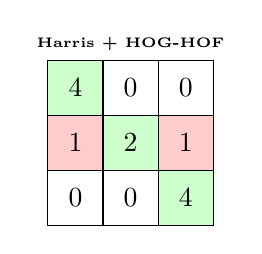
\begin{tikzpicture}[scale=0.7]
            \draw[fill=green!20] (0,2) rectangle (1,3) node[pos=.5] {4};
            \draw[fill=white] (1,2) rectangle (2,3) node[pos=.5] {0};
            \draw[fill=white] (2,2) rectangle (3,3) node[pos=.5] {0};
            
            \draw[fill=red!20] (0,1) rectangle (1,2) node[pos=.5] {1};
            \draw[fill=green!20] (1,1) rectangle (2,2) node[pos=.5] {2};
            \draw[fill=red!20] (2,1) rectangle (3,2) node[pos=.5] {1};
            
            \draw[fill=white] (0,0) rectangle (1,1) node[pos=.5] {0};
            \draw[fill=white] (1,0) rectangle (2,1) node[pos=.5] {0};
            \draw[fill=green!20] (2,0) rectangle (3,1) node[pos=.5] {4};
            
            \node at (1.5,3.3) {\tiny \textbf{Harris + HOG-HOF}};
         \end{tikzpicture}
         \caption{Accuracy: 0.83}
     \end{subfigure}
     
     \caption{Confusion Matrices για συνδυασμούς του ανιχνευτή Harris (0: Handclapping, 1: Running, 2: Walking).}
     \label{fig:confusion_matrices}
\end{figure}

\begin{figure}[H]
     \centering
     % --- Confusion Matrix 1: MultiScale-Harris + HOG ---
     \begin{subfigure}[b]{0.3\textwidth}
         \centering
         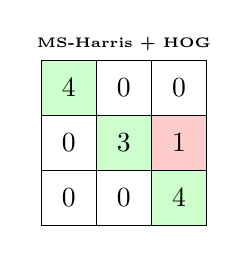
\begin{tikzpicture}[scale=0.7]
            \draw[fill=green!20] (0,2) rectangle (1,3) node[pos=.5] {4};
            \draw[fill=white] (1,2) rectangle (2,3) node[pos=.5] {0};
            \draw[fill=white] (2,2) rectangle (3,3) node[pos=.5] {0};
            
            \draw[fill=white] (0,1) rectangle (1,2) node[pos=.5] {0};
            \draw[fill=green!20] (1,1) rectangle (2,2) node[pos=.5] {3};
            \draw[fill=red!20] (2,1) rectangle (3,2) node[pos=.5] {1};
            
            \draw[fill=white] (0,0) rectangle (1,1) node[pos=.5] {0};
            \draw[fill=white] (1,0) rectangle (2,1) node[pos=.5] {0};
            \draw[fill=green!20] (2,0) rectangle (3,1) node[pos=.5] {4};
            
            \node at (1.5,3.3) {\tiny \textbf{MS-Harris + HOG}};
         \end{tikzpicture}
         \caption{Accuracy: 0.92}
     \end{subfigure}
     \hfill
     % --- Confusion Matrix 2: MultiScale-Harris + HOF ---
     \begin{subfigure}[b]{0.3\textwidth}
         \centering
         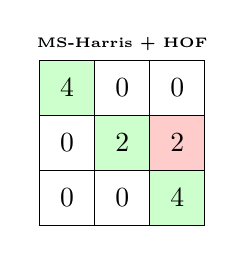
\begin{tikzpicture}[scale=0.7]
            \draw[fill=green!20] (0,2) rectangle (1,3) node[pos=.5] {4};
            \draw[fill=white] (1,2) rectangle (2,3) node[pos=.5] {0};
            \draw[fill=white] (2,2) rectangle (3,3) node[pos=.5] {0};
            
            \draw[fill=white] (0,1) rectangle (1,2) node[pos=.5] {0};
            \draw[fill=green!20] (1,1) rectangle (2,2) node[pos=.5] {2};
            \draw[fill=red!20] (2,1) rectangle (3,2) node[pos=.5] {2};
            
            \draw[fill=white] (0,0) rectangle (1,1) node[pos=.5] {0};
            \draw[fill=white] (1,0) rectangle (2,1) node[pos=.5] {0};
            \draw[fill=green!20] (2,0) rectangle (3,1) node[pos=.5] {4};
            
            \node at (1.5,3.3) {\tiny \textbf{MS-Harris + HOF}};
         \end{tikzpicture}
         \caption{Accuracy: 0.83}
     \end{subfigure}
     \hfill
     % --- Confusion Matrix 3: MultiScale-Harris + HOG-HOF ---
     \begin{subfigure}[b]{0.3\textwidth}
         \centering
         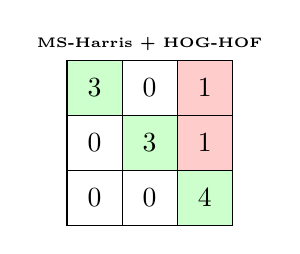
\begin{tikzpicture}[scale=0.7]
            \draw[fill=green!20] (0,2) rectangle (1,3) node[pos=.5] {3};
            \draw[fill=white] (1,2) rectangle (2,3) node[pos=.5] {0};
            \draw[fill=red!20] (2,2) rectangle (3,3) node[pos=.5] {1};
            
            \draw[fill=white] (0,1) rectangle (1,2) node[pos=.5] {0};
            \draw[fill=green!20] (1,1) rectangle (2,2) node[pos=.5] {3};
            \draw[fill=red!20] (2,1) rectangle (3,2) node[pos=.5] {1};
            
            \draw[fill=white] (0,0) rectangle (1,1) node[pos=.5] {0};
            \draw[fill=white] (1,0) rectangle (2,1) node[pos=.5] {0};
            \draw[fill=green!20] (2,0) rectangle (3,1) node[pos=.5] {4};
            
            \node at (1.5,3.3) {\tiny \textbf{MS-Harris + HOG-HOF}};
         \end{tikzpicture}
         \caption{Accuracy: 0.83}
     \end{subfigure}
     
     \caption{Confusion Matrices για συνδυασμούς του ανιχνευτή MultiScale-Harris (0: Handclapping, 1: Running, 2: Walking).}
     \label{fig:confusion_matrices_multiscale}
\end{figure}

\begin{figure}[H]
     \centering
     % --- Confusion Matrix 1: Gabor + HOG ---
     \begin{subfigure}[b]{0.3\textwidth}
         \centering
         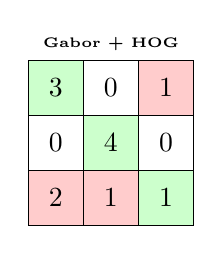
\begin{tikzpicture}[scale=0.7]
            \draw[fill=green!20] (0,2) rectangle (1,3) node[pos=.5] {3};
            \draw[fill=white] (1,2) rectangle (2,3) node[pos=.5] {0};
            \draw[fill=red!20] (2,2) rectangle (3,3) node[pos=.5] {1};
            
            \draw[fill=white] (0,1) rectangle (1,2) node[pos=.5] {0};
            \draw[fill=green!20] (1,1) rectangle (2,2) node[pos=.5] {4};
            \draw[fill=white] (2,1) rectangle (3,2) node[pos=.5] {0};
            
            \draw[fill=red!20] (0,0) rectangle (1,1) node[pos=.5] {2};
            \draw[fill=red!20] (1,0) rectangle (2,1) node[pos=.5] {1};
            \draw[fill=green!20] (2,0) rectangle (3,1) node[pos=.5] {1};
            
            \node at (1.5,3.3) {\tiny \textbf{Gabor + HOG}};
         \end{tikzpicture}
         \caption{Accuracy: 0.67}
     \end{subfigure}
     \hfill
     % --- Confusion Matrix 2: Gabor + HOF ---
     \begin{subfigure}[b]{0.3\textwidth}
         \centering
         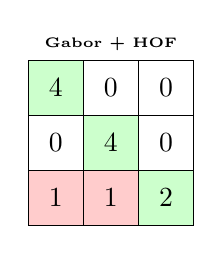
\begin{tikzpicture}[scale=0.7]
            \draw[fill=green!20] (0,2) rectangle (1,3) node[pos=.5] {4};
            \draw[fill=white] (1,2) rectangle (2,3) node[pos=.5] {0};
            \draw[fill=white] (2,2) rectangle (3,3) node[pos=.5] {0};
            
            \draw[fill=white] (0,1) rectangle (1,2) node[pos=.5] {0};
            \draw[fill=green!20] (1,1) rectangle (2,2) node[pos=.5] {4};
            \draw[fill=white] (2,1) rectangle (3,2) node[pos=.5] {0};
            
            \draw[fill=red!20] (0,0) rectangle (1,1) node[pos=.5] {1};
            \draw[fill=red!20] (1,0) rectangle (2,1) node[pos=.5] {1};
            \draw[fill=green!20] (2,0) rectangle (3,1) node[pos=.5] {2};
            
            \node at (1.5,3.3) {\tiny \textbf{Gabor + HOF}};
         \end{tikzpicture}
         \caption{Accuracy: 0.83}
     \end{subfigure}
     \hfill
     % --- Confusion Matrix 3: Gabor + HOG-HOF ---
     \begin{subfigure}[b]{0.3\textwidth}
         \centering
         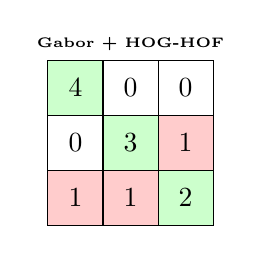
\begin{tikzpicture}[scale=0.7]
            \draw[fill=green!20] (0,2) rectangle (1,3) node[pos=.5] {4};
            \draw[fill=white] (1,2) rectangle (2,3) node[pos=.5] {0};
            \draw[fill=white] (2,2) rectangle (3,3) node[pos=.5] {0};
            
            \draw[fill=white] (0,1) rectangle (1,2) node[pos=.5] {0};
            \draw[fill=green!20] (1,1) rectangle (2,2) node[pos=.5] {3};
            \draw[fill=red!20] (2,1) rectangle (3,2) node[pos=.5] {1};
            
            \draw[fill=red!20] (0,0) rectangle (1,1) node[pos=.5] {1};
            \draw[fill=red!20] (1,0) rectangle (2,1) node[pos=.5] {1};
            \draw[fill=green!20] (2,0) rectangle (3,1) node[pos=.5] {2};
            
            \node at (1.5,3.3) {\tiny \textbf{Gabor + HOG-HOF}};
         \end{tikzpicture}
         \caption{Accuracy: 0.75}
     \end{subfigure}
     
     \caption{Confusion Matrices για συνδυασμούς του ανιχνευτή Gabor (0: Handclapping, 1: Running, 2: Walking).}
     \label{fig:confusion_matrices_gabor}
\end{figure}


\section*{Μέρος 3: Ταξινόμηση video με χρήση προεκπαιδευμένων βαθιών νευρωνικών δικτύων}
\subsection*{3.1 Αναγνώριση Δράσεων με 2D CNN}

\hspace{0.6cm}Στο μέρος αυτό αξιοποιείται το προ-εκπαιδευμένο δίκτυο \texttt{MobileNet\_V3\_Small} ως εξαγωγέας χωρικών χαρακτηριστικών από το dataset UCF11, το οποίο αποτελεί ένα σημαντικά πιο απαιτητικό σύνολο δεδομένων σε σχέση με το KTH. Σε αντίθεση με το ελεγχόμενο περιβάλλον και τις απλές δράσεις του KTH, το UCF11 περιλαμβάνει μεγαλύτερο πλήθος κλάσεων με πιο σύνθετες και άναρχες κινήσεις σε έγχρωμα βίντεο. Επιπλέον, εισάγει προκλήσεις όπως η έντονη δραστηριότητα στο υπόβαθρο και η ταυτόχρονη εμφάνιση πολλαπλών υποκειμένων στο ίδιο πλάνο, γεγονός που καθιστά την εξαγωγή αντιπροσωπευτικών χαρακτηριστικών πολύ πιο δυσχερή.

Η χρονική διάσταση του βίντεο αντιμετωπίζεται μέσω \textit{average pooling} επί των περιγραφητών όλων των πλαισίων. Η προσέγγιση αυτή παράγει έναν ενιαίο περιγραφητή ανά βίντεο που κωδικοποιεί τη μέση χωρική πληροφορία της δράσης καθόλη τη διάρκειά της. Επισημαίνεται ότι η διαδικασία αυτή στερείται της πληροφορίας για τη σχετική χρονική σειρά εμφάνισης των χαρακτηριστικών, καθώς αντιμετωπίζει το βίντεο ως μια στατική συλλογή πλαισίων (bag-of-frames) όπου η χρονική αλληλουχία δεν λαμβάνεται υπόψη.

Για την τελική κατηγοριοποίηση χρησιμοποιείται SVM ταξινομητής με γραμμικό πυρήνα, όπως ορίζεται από τις προδιαγραφές της άσκησης.

\subsubsection*{Συνάρτηση \texttt{FeatureExtractionCNN2D}}
Η συνάρτηση \texttt{FeatureExtractionCNN2D} διαχειρίζεται την εξαγωγή χαρακτηριστικών, θέτοντας το δίκτυο σε \texttt{eval()} mode. Ο διαχωρισμός των δεδομένων πραγματοποιείται με τη χρήση του flag \texttt{is\_train} βάσει του αρχείου \texttt{training\_videos.txt}. Η έξοδος είναι ένα λεξικό (\texttt{features}) με κλειδιά \texttt{train\_desc}, \texttt{test\_desc}, \texttt{train\_labels} και \texttt{test\_labels}, όπου οι περιγραφητές αποθηκεύονται ως λίστες διανυσμάτων.


\subsection*{3.2 Αναγνώριση Δράσεων με 3D CNN}

Η συνάρτηση FEatureExtractionCNN3D επιστρέφει ένα λεξικό features με την δομή που έχουμε ήδη περιγράψει. Σε αντίθεση με το 2D CNN (οπού η αλληλουχία χάνεται λόγω \textit{average pooling}), το 3D CNN επεξεργάζεται απευθείας χωροχρονικούς όγκους. Αυτό του επιτρέπει να κωδικοποιεί εγγενώς την κατεύθυνση, την ταχύτητα και τη δυναμική της κίνησης στον χρόνο, παράγοντας πολύ πιο πλούσιους περιγραφητές.
Τέλος για την προσαρμογή βίντεο μεταβλητού μεγέθους στον σταθερό τανυστή, η μέθοδος interpolation προτιμήθηκε από την απλής υπο/υπερ-δειγματοληψίας. Με αυτόν τον τρόπο οι νέες τιμές λαμβάνουν υπόψη όλο τον χωροχρονικό περίγυρο, διατηρώντας την κίνηση ομαλή και αποτρέποντας το φαινόμενο του aliasing (απότομα σπασίματα στην κίνηση).


\subsection*{3.2.4 Σύγκριση και Ερμηνεία Αποτελεσμάτων (2D έναντι 3D CNN)}

Στον Table 5 συνοψίζονται οι επιδόσεις των τριών προσεγγίσεων βαθιάς μάθησης που εφαρμόστηκαν στο dataset UCF11.

\begin{table}[h!]
\centering
\begin{tabular}{@{}lc@{}}
\toprule
\textbf{Αρχιτεκτονική \& Μέθοδος Εξαγωγής} & \textbf{Ακρίβεια (Accuracy)} \\ \midrule
2D CNN (MobileNetV3) - Average Pooling όλων των frames        & \textbf{0.988} \\
3D CNN (X3D) - Συμπίεση όλου του βίντεο σε 4 frames (Baseline)& 0.964          \\
3D CNN (X3D) - Επεξεργασία ανά 4 frames \& Avg Pooling (Alt)  & \textbf{0.988} \\ \bottomrule
\end{tabular}
\caption{Αποτελέσματα Accuracy CNN μοντέλων στο UCF11}
\label{tab:cnn_results}
\end{table}

\subsubsection*{Ανάλυση Επιδόσεων}

\begin{itemize}
    \item \textbf{Κυριαρχία της Χωρικής Πληροφορίας (2D CNN):} Η εξαιρετικά υψηλή απόδοση του 2D CNN (98.8\%) καταδεικνύει ότι στο UCF11 η χωρική πληροφορία και το περιεχόμενο του υποβάθρου είναι ισχυρότατα διακριτικά στοιχεία. Για παράδειγμα, η παρουσία μιας πισίνας, ενός ποδηλάτου ή μιας μπάλας μπάσκετ στο πλάνο επιτρέπει στο μοντέλο να ταξινομήσει σωστά τη δράση, ακόμη και χωρίς να κατανοεί την εξέλιξη της κίνησης στον χρόνο.
    
    \item \textbf{Απώλεια Πληροφορίας στο Baseline 3D CNN:} Η αρχική προσέγγιση (Baseline 3D), όπου ολόκληρο το βίντεο συμπιέστηκε σε έναν τανυστή μόλις $T=4$ καρέ μέσω trilinear interpolation, παρουσίασε τη χαμηλότερη επίδοση (96.4\%). Αυτό συμβαίνει διότι η ακραία υποδειγματοληψία καταστρέφει την ομαλότητα της κίνησης και αφαιρεί κρίσιμες ενδιάμεσες πόζες της δράσης. Το 3D δίκτυο, το οποίο είναι σχεδιασμένο να αναζητά χωροχρονικά μοτίβα, τροφοδοτείται με σπασμωδική πληροφορία, οδηγώντας σε αυξημένη σύγχυση, ιδίως στην κλάση \textit{walking} (η οποία συγχέεται με \textit{biking} και \textit{swing}). Σε μια απόπειρα ερμηνείας αυτού του φαινομένου μπορούμε να πούμε ότι η ακραία χρονική συμπίεση των 4 καρέ αλλοιώνει τον φυσικό ρυθμό της βάδισης, με αποτέλεσμα το δίκτυο να την εκλαμβάνει απλώς ως μια γενικευμένη περιοδική κίνηση, συγχέοντάς την εύκολα με την εξίσου επαναλαμβανόμενη δυναμική του πεταλιού (biking) ή της αιώρησης (swing).
    
    \item \textbf{Η Εναλλακτική Βελτίωση (Alternative 3D CNN):} Για να αντιμετωπιστεί το παραπάνω πρόβλημα, εισήχθη μια εναλλακτική προσέγγιση: το βίντεο χωρίστηκε σε μικρά, διαδοχικά clips των 4 καρέ. Τα χαρακτηριστικά εξήχθησαν για κάθε clip ξεχωριστά, μέσω του 3D CNN και στη συνέχεια εφαρμόστηκε \textit{Average Pooling} για την παραγωγή ενός ενιαίου περιγραφητή. Η μέθοδος αυτή ανέκαμψε την ακρίβεια στο 98.8\%, εξαλείφοντας τα σφάλματα του Baseline. Επέτρεψε στο X3D να επεξεργαστεί σωστά την τοπική δυναμική της κίνησης σε κάθε clip, ενώ η τελική συσσώρευση συνόψισε τη συνολική δομή του βίντεο.
\end{itemize}

\textbf{Συμπέρασμα:} Η ισοπαλία (98.8\%) μεταξύ του 2D CNN και της βελτιωμένης 3D προσέγγισης υποδηλώνει ένα άνω όριο στην απόδοση για το συγκεκριμένο υποσύνολο του UCF11. Τα χωρικά χαρακτηριστικά από μόνα τους είναι ήδη αρκετά για την επίλυση του προβλήματος, αλλά όταν χρησιμοποιείται μια 3D αρχιτεκτονική, είναι απολύτως αναγκαία η σωστή χρονική δειγματοληψία για να μην υποβαθμιστεί η απόδοση.

\begin{figure}[H]
     \centering
     % --- Confusion Matrix 1: 2D CNN ---
     \begin{subfigure}[b]{0.32\textwidth}
         \centering
         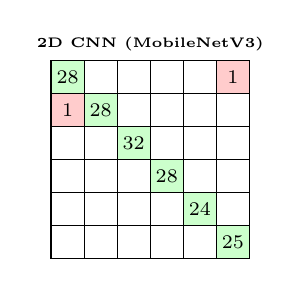
\begin{tikzpicture}[scale=0.42]
            % Main Diagonal (Correct Predictions)
            \foreach \x/\z in {0/28, 1/28, 2/32, 3/28, 4/24, 5/25}
                \draw[fill=green!20] (\x, 5-\x) rectangle (\x+1, 6-\x) node[pos=.5] {\scriptsize \z};
            
            % Errors
            \draw[fill=red!20] (5, 5) rectangle (6, 6) node[pos=.5] {\scriptsize 1};
            \draw[fill=red!20] (0, 4) rectangle (1, 5) node[pos=.5] {\scriptsize 1};
            
            % Grid
            \foreach \i in {0,...,5}
                \foreach \j in {0,...,5}
                    \draw (\i, \j) rectangle (\i+1, \j+1);

            \node at (3,6.5) {\tiny \textbf{2D CNN (MobileNetV3)}};
         \end{tikzpicture}
         \caption{Acc: 0.988}
     \end{subfigure}
     \hfill
     % --- Confusion Matrix 2: 3D CNN (Baseline) ---
     \begin{subfigure}[b]{0.32\textwidth}
         \centering
         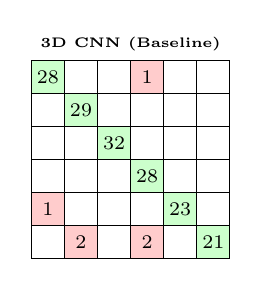
\begin{tikzpicture}[scale=0.42]
            \foreach \x/\z in {0/28, 1/29, 2/32, 3/28, 4/23, 5/21}
                \draw[fill=green!20] (\x, 5-\x) rectangle (\x+1, 6-\x) node[pos=.5] {\scriptsize \z};
            
            \draw[fill=red!20] (3, 5) rectangle (4, 6) node[pos=.5] {\scriptsize 1};
            \draw[fill=red!20] (0, 1) rectangle (1, 2) node[pos=.5] {\scriptsize 1};
            \draw[fill=red!20] (1, 0) rectangle (2, 1) node[pos=.5] {\scriptsize 2};
            \draw[fill=red!20] (3, 0) rectangle (4, 1) node[pos=.5] {\scriptsize 2};

            \foreach \i in {0,...,5}
                \foreach \j in {0,...,5}
                    \draw (\i, \j) rectangle (\i+1, \j+1);

            \node at (3,6.5) {\tiny \textbf{3D CNN (Baseline)}};
         \end{tikzpicture}
         \caption{Acc: 0.964}
     \end{subfigure}
     \hfill
     % --- Confusion Matrix 3: 3D CNN (Alternative) ---
     \begin{subfigure}[b]{0.32\textwidth}
         \centering
         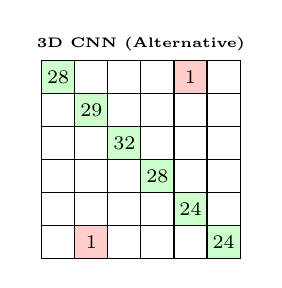
\begin{tikzpicture}[scale=0.42]
            \foreach \x/\z in {0/28, 1/29, 2/32, 3/28, 4/24, 5/24}
                \draw[fill=green!20] (\x, 5-\x) rectangle (\x+1, 6-\x) node[pos=.5] {\scriptsize \z};
            
            \draw[fill=red!20] (4, 5) rectangle (5, 6) node[pos=.5] {\scriptsize 1};
            \draw[fill=red!20] (1, 0) rectangle (2, 1) node[pos=.5] {\scriptsize 1};

            \foreach \i in {0,...,5}
                \foreach \j in {0,...,5}
                    \draw (\i, \j) rectangle (\i+1, \j+1);

            \node at (3,6.5) {\tiny \textbf{3D CNN (Alternative)}};
         \end{tikzpicture}
         \caption{Acc: 0.988}
     \end{subfigure}
     \caption{Confusion Matrices για τις τρεις προσεγγίσεις CNN στο UCF11.}
\end{figure}
\newpage
\section*{Πηγές}
Μαραγκός Π. Ανάλυση Εικόνων και Όραση Υπολογιστών. Ε.Μ.Π. 2014.
\end{document}
